\documentclass[a4paper]{article}
\usepackage[pdftex]{hyperref}
\usepackage[latin1]{inputenc}
\usepackage[english]{babel}
\usepackage{a4wide}
\usepackage{amsmath}
\usepackage{amssymb}
\usepackage{algorithmic}
\usepackage{algorithm}
\usepackage{ifthen}
\usepackage{listings}
\usepackage{hyperref}
\usepackage{minted}
% move the asterisk at the right position
\lstset{basicstyle=\ttfamily,tabsize=4,literate={*}{${}^*{}$}1}
%\lstset{language=C,basicstyle=\ttfamily}
%\usepackage{moreverb}
\usepackage{palatino}
\usepackage{multicol}
\usepackage{tabularx}
%\usepackage{comment}
\usepackage{verbatim}
\usepackage{color}

%% pdflatex?
\newif\ifpdf
\ifx\pdfoutput\undefined
\pdffalse % we are not running PDFLaTeX
\else
\pdfoutput=1 % we are running PDFLaTeX
\pdftrue
\fi
\ifpdf
\usepackage[pdftex]{graphicx}
\else
\usepackage{graphicx}
\fi
\ifpdf
\DeclareGraphicsExtensions{.pdf, .jpg}
\else
\DeclareGraphicsExtensions{.eps, .jpg}
\fi

\parindent=0cm
\parskip=0cm

\setlength{\columnseprule}{0.4pt}
\addtolength{\columnsep}{2pt}

\addtolength{\textheight}{5.5cm}
\addtolength{\topmargin}{-26mm}
\pagestyle{empty}

%%
%% Sheet setup
%% 
\newcommand{\coursename}{Computer Architecture and Programming Languages}
\newcommand{\courseno}{CO20-320241}
 
\newcommand{\sheettitle}{Homework}
\newcommand{\mytitle}{}
\newcommand{\mytoday}{\textcolor{blue}{November 25th}, 2019}

% Current Assignment number
\newcounter{assignmentno}
\setcounter{assignmentno}{10}

% Current Problem number, should always start at 1
\newcounter{problemno}
\setcounter{problemno}{1}

%%
%% problem and bonus environment
%%
\newcounter{probcalc}
\newcommand{\problem}[2]{
  \pagebreak[2]
  \setcounter{probcalc}{#2}
  ~\\
  {\large \textbf{Problem \textcolor{blue}{\arabic{assignmentno}}.\textcolor{blue}{\arabic{problemno}}} \hspace{0.2cm}\textit{#1}} \refstepcounter{problemno}\vspace{2pt}\\}

\newcommand{\bonus}[2]{
  \pagebreak[2]
  \setcounter{probcalc}{#2}
  ~\\
  {\large \textbf{Bonus Problem \textcolor{blue}{\arabic{assignmentno}}.\textcolor{blue}{\arabic{problemno}}} \hspace{0.2cm}\textit{#1}} \refstepcounter{problemno}\vspace{2pt}\\}

%% some counters  
\newcommand{\assignment}{\arabic{assignmentno}}

%% solution  
\newcommand{\solution}{\pagebreak[2]{\bf Solution:}\\}

%% Hyperref Setup
\hypersetup{pdftitle={Homework \assignment},
  pdfsubject={\coursename},
  pdfauthor={},
  pdfcreator={},
  pdfkeywords={Computer Architecture and Programming Languages},
  %  pdfpagemode={FullScreen},
  %colorlinks=true,
  %bookmarks=true,
  %hyperindex=true,
  bookmarksopen=false,
  bookmarksnumbered=true,
  breaklinks=true,
  %urlcolor=darkblue
  urlbordercolor={0 0 0.7}
}

\begin{document}
\coursename \hfill Course: \courseno\\
Jacobs University Bremen \hfill \mytoday\\
\textcolor{blue}{Arsenij Percov}\hfill
\vspace*{0.3cm}\\
\begin{center}
{\Large \sheettitle{} \textcolor{blue}{\assignment}\\}
\end{center}

\problem{}{0}
\solution
Controls lines are necessary to select input type for shared elements, like for example ALU, also they are needed to define the format of the input(R-type or I-type or J-type for example) and  like for example ALUsrc. They communicate with multiplexers, and dictate which input to select as output for multiplexer, which are used to direct the result, and choose some operation-specific manipulations.
\\
\problem{}{0}
\solution

This is the datapath that is able to execute both add, and addi.\\
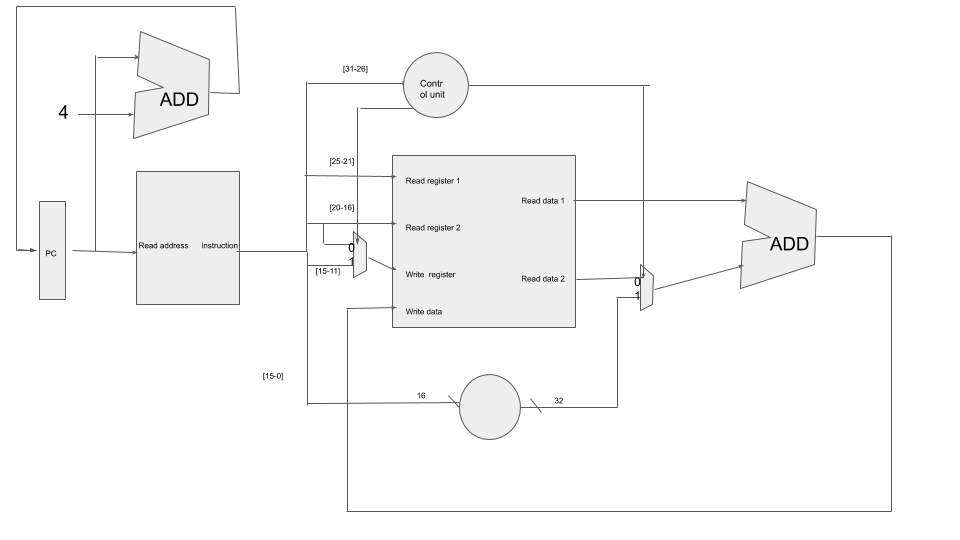
\includegraphics[scale=0.5]{datapath.png}
\\\\
Here is the path for add(red arrows are used in the example):\\
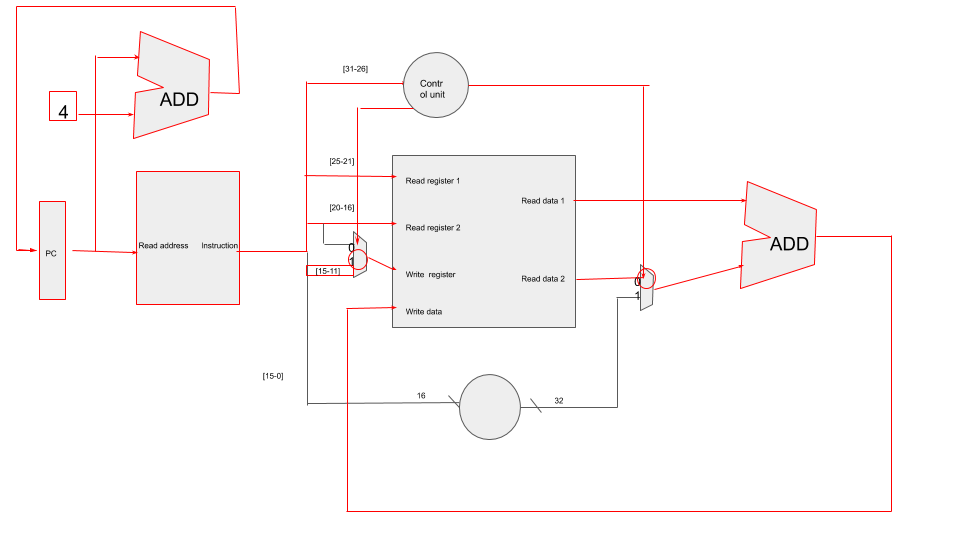
\includegraphics[scale=0.5]{datapath-add.png}
\\\\
Datapath for addi, reads 20-16 bits as write register with help of multiplexer, and control line, and later it uses 15-00 extended to 32 bits as parameter for add, and later stores it in write data.
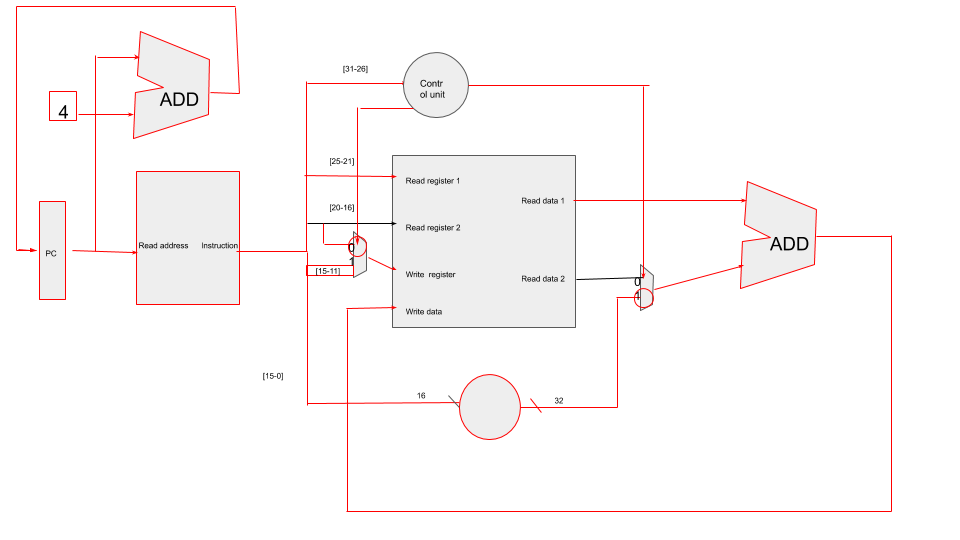
\includegraphics[scale=0.5]{data.png}

\problem{}{0}
\solution
Find the longest instruction paths.\\
a)Out of all possible paths for instructions, this one is the longest one. We start operation, go throw register, from where we through multiplex send output to ALU, do the operation, and select to return it to Regs to write it there, using multiplex.
I-mem, Regs, Mux, ALU, Mux, Regs \\
450 + 250 + 30 + 120 + 30 + 250 = 1130ps\\
\\
b) 
The data goes from I-Mem to sign extend and Regs, however since Regs takes longer time, and instructions are parallel, then we only include Regs to calculations, then we go to AlU, adding the sign extend, and finally we store data to memory in D-Mem.\\
I-Mem, RegF, ALU, D-Mem\\
450 + 250 + 120 + 350 = 1170ps\\\\
c)We need to find the longest instruction among all of these in the datapath designed to support all of them.
Longest time for sw is 1170, add is ALU instruction, and longest ALU instruction takes 1130ps, so we only need to find beq and lw longest times.
\\
beq =  I-Mem + RegF + Mux + ALU + Mux = 450+250+30+120+30=880 ps\\
lw = I-Mem + RegF + ALU + D-Mem + Mux + RegF = 450 + 250 + 120 + 350 +30 +250 = 1450ps.
\\Therefore, lw is the longest instruction with the clock cycle time of 1450 ps.


\end{document} 